% ****** Start of file apssamp.tex ******
%
%   This file is part of the APS files in the REVTeX 4.2 distribution.
%   Version 4.2a of REVTeX, December 2014
%
%   Copyright (c) 2014 The American Physical Society.
%
%   See the REVTeX 4 README file for restrictions and more information.
%
% TeX'ing this file requires that you have AMS-LaTeX 2.0 installed
% as well as the rest of the prerequisites for REVTeX 4.2
%
% See the REVTeX 4 README file
% It also requires running BibTeX. The commands are as follows:
%
%  1)  latex apssamp.tex
%  2)  bibtex apssamp
%  3)  latex apssamp.tex
%  4)  latex apssamp.tex
%
\documentclass[%
 % reprint,
10pt,
superscriptaddress,
% twocolumn,
%groupedaddress,
%unsortedaddress,
%runinaddress,
%frontmatterverbose,
%preprint,
%preprintnumbers,
%nofootinbib,
%nobibnotes,
%bibnotes,
 amsmath,amssymb,
 aps,prx,
%pra,
%prb,
%rmp,
%prstab,
%prstper,
%floatfix,
]{revtex4-2}

\usepackage{graphicx}% Include figure files
\usepackage{dcolumn}% Align table columns on decimal point
\usepackage{bm}% bold math
\usepackage{xcolor}
\usepackage{hyperref}% add hypertext capabilities
\usepackage{siunitx}% SI units
\usepackage{physics}
\usepackage[utf8]{inputenc}
\usepackage[T1]{fontenc}
\usepackage{lmodern}
\usepackage{amsmath,amsfonts,amssymb}


\AtBeginDocument{\renewcommand*{\d}{\mathop{\kern0pt\mathrm{d}}\!{}}}
\graphicspath{{Figures/}} % set default figure path to figures/, if we store figure files in figures/, we only need to put file name in \includegraphics{filename.pdf}. For supported formats, e.g. pdf and jpg, we can omit the extensions. This enhances the readability of the source.

% Some formatting guidelines
% 1. Start a new line (\n) for each sentence. This is good for synctex (click pdf and find the line in tex), and also good for Git when comparing versions.
% 2. Communicate thoughts in comments. For example, if you think a figure of something is needed but missing some where, put a comment and describe the needs.
% 3. Colored text: I use red text to emphasize that the claim is not fully backed by our results. The wording may be modified in the future.
% 4. Figure crossref: at the beginning of a sentence, use "Figure~\ref{}". Otherwise, use "Fig.~\ref{}". Note that the "~" is to prevent line breaking in the middle of the crossref.

% Some content problems that need to be fixed
% 1. Same quantities are referred to in different notations, e.g. \tau^* and \tilde{\tau}, x and y, \tilde{D} and D_A



\begin{document}

\preprint{APS/123-QED}

\title{Active Nematics at Bifurcations}% Force line breaks with \\



\author{Zhengyang Liu}
\author{Claire Doré}
\affiliation{Laboratoire Gulliver, UMR 7083 CNRS, ESPCI Paris, PSL Research University, 75005 Paris, France.}

\author{Antonio Tavera-Vazquez}
\affiliation{Laboratoire Gulliver, UMR 7083 CNRS, ESPCI Paris, PSL Research University, 75005 Paris, France.}
\affiliation{Pritzker School of Molecular Engineering, University of Chicago, Chicago, IL 60637, USA.}

\author{Teresa Lopez-Leon}
\affiliation{Laboratoire Gulliver, UMR 7083 CNRS, ESPCI Paris, PSL Research University, 75005 Paris, France.}
\date{\today}
% It is always \today, today,
%  but any date may be explicitly specified

%\keywords{Suggested keywords}%Use showkeys class option if keyword
                              %display desired
\maketitle

\begin{figure}[!h]
    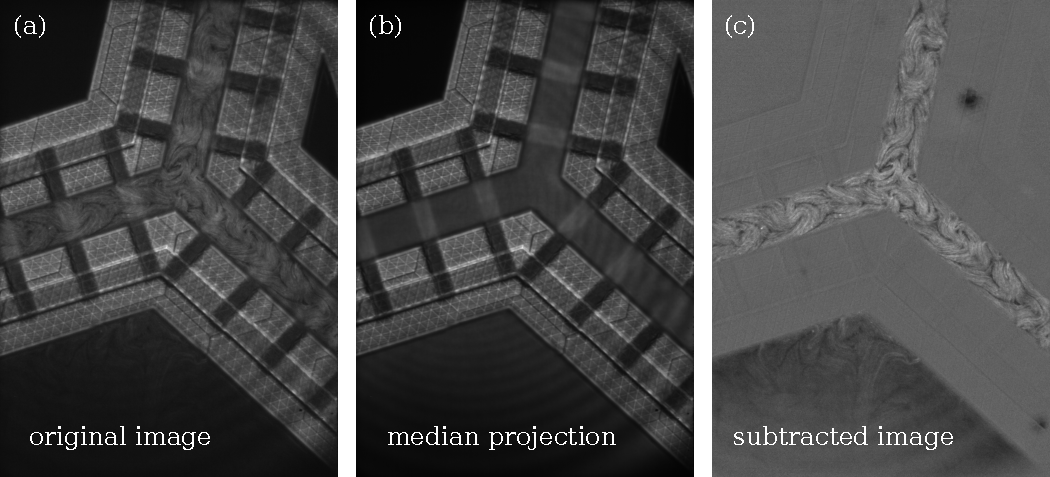
\includegraphics[width=\textwidth]{a1-remove-background}
    \caption{
    \textbf{Image processing -- remove background.}
    }
    \label{fig:remove-background}
\end{figure}

\begin{figure}[!h]
    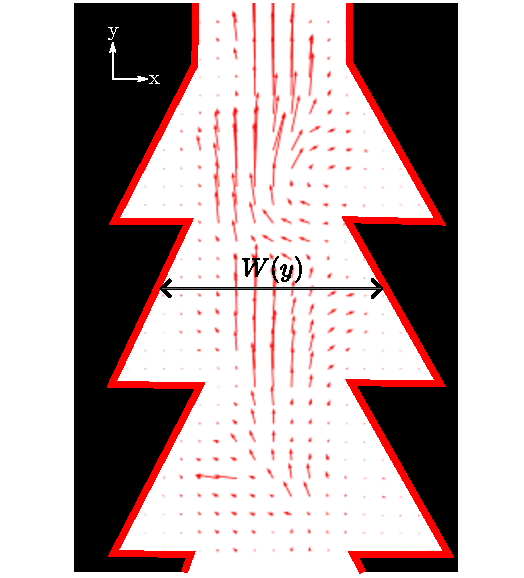
\includegraphics[width=0.4\textwidth]{a2-flowrate-channel-width}
    \caption{
    \textbf{Compute flow rate from PIV data -- the definition of channel width.}
    }
    \label{fig:flowrate-channel-width}
\end{figure}

\begin{figure}[!h]
    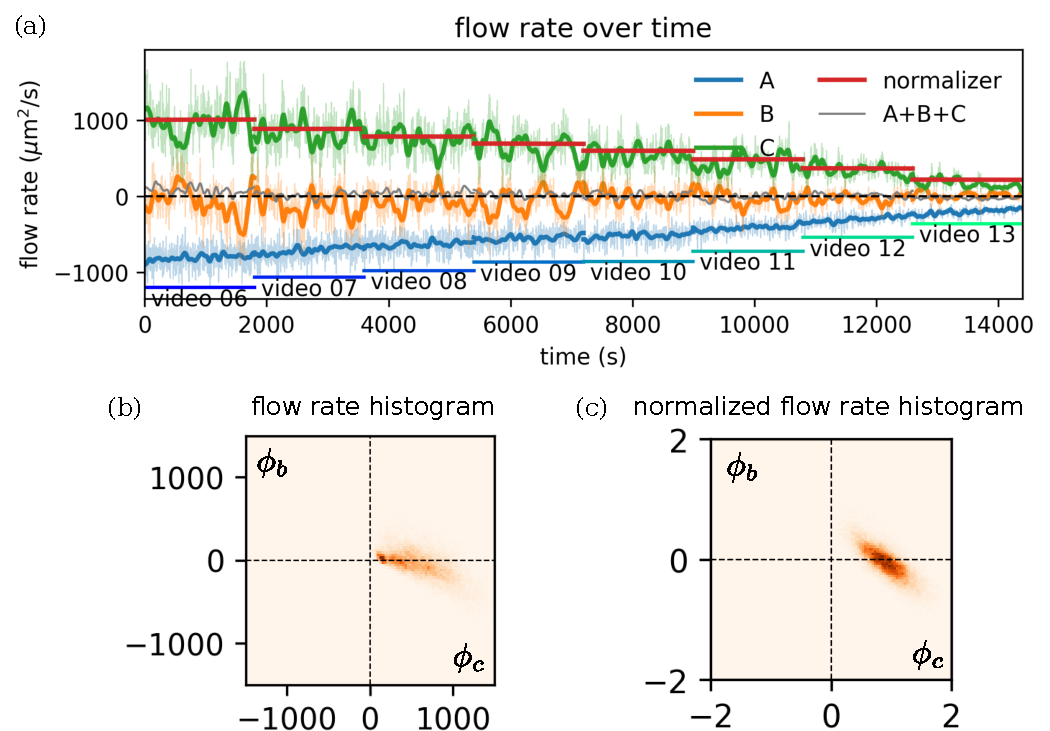
\includegraphics[width=\textwidth]{a3-normalization-of-flow-rate}
    \caption{
    \textbf{Normalizing the flow rate data to account for the long time variation due to constantly decreasing activity.}
    }
    \label{fig:normalization-of-flow-rate}
\end{figure}

\begin{figure}[!h]
    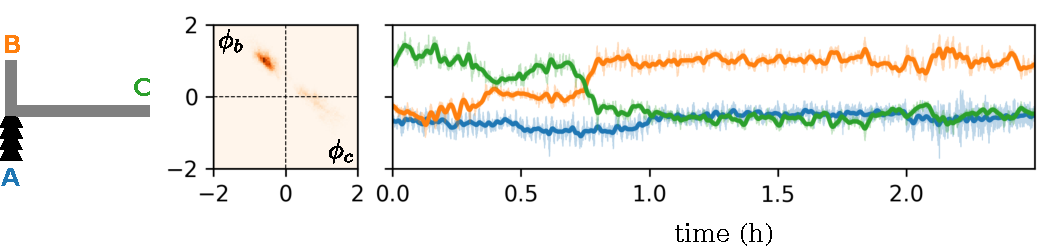
\includegraphics[width=\textwidth]{a4-angle-length-competition}
    \caption{
    \textbf{Competition between angle and straight channel length.}
    }
    \label{fig:angle-length-competition}
\end{figure}

\begin{figure}[!h]
    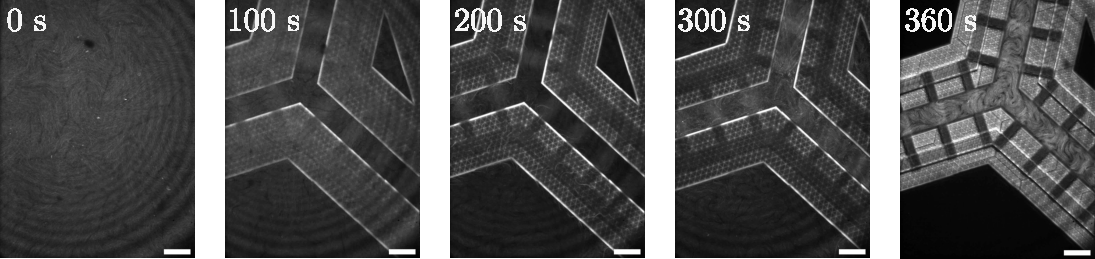
\includegraphics[width=\textwidth]{a5-apply-grid}
    \caption{
    \textbf{Applying bifurcation channels to the interfacial microtubule-kinesin system.}
    }
    \label{fig:apply-grid}
\end{figure}

\begin{figure}[!h]
    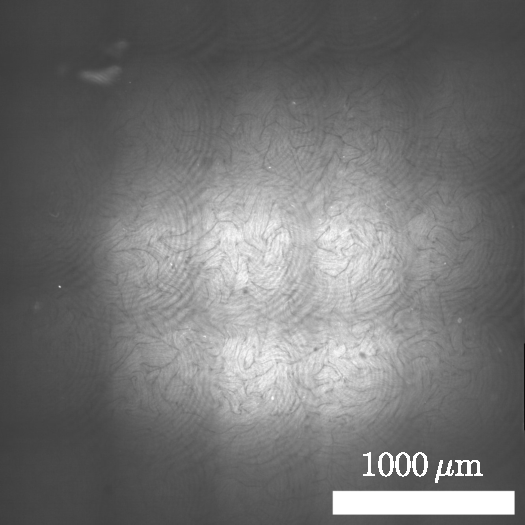
\includegraphics[width=0.5\textwidth]{a6-curved-interface}
    \caption{
    \textbf{Confocal image of the microtubule-kinesin system interface, showing that the interface is slightly curved due to the competition between surface tension and gravity.}
    }
    \label{fig:curved-interface}
\end{figure}

\end{document}
%
% ****** End of file apssamp.tex ******